\section{Dağılım Türleri}
Bir olasılık dağılımı bir rassal olayın ortaya çıkabilmesi için değerleri ve olasılıkları tanımlar. Değerler olay için mümkün olan tüm sonuçları kapsamalıdır ve olasılıkların toplamı bire eşit olmalıdır. Sonuçların birbirinden ayrı olduğu ve devamlılık arz etmeyen dağılımlara kesikli (discrete) dağılım denir. 

\begin{figure}[h]
    \centering
    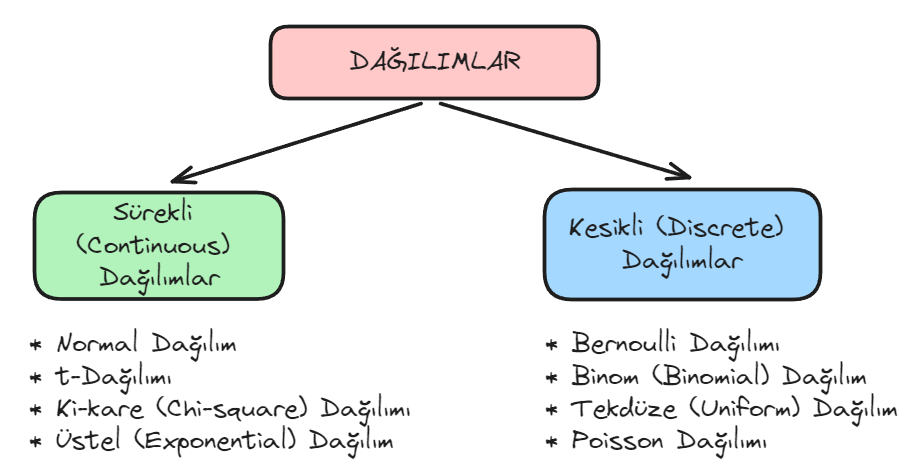
\includegraphics[width=1\textwidth]{images/types_of_distribution.png}
    \caption{Dağılım türleri.}
    \label{fig:enter-label}
\end{figure}

\newpage

\subsection{Normal Dağılım}
Gauss dağılımı olarak da bilinir. Belirli bir ortalama değer etrafında simetrik bir şekilde dağılan bir olasılık dağılımıdır. Çan eğrisi olarak adlandırılan bir görünüme sahiptir.

\[f(x | \mu, \sigma^2) = \frac{1}{\sqrt{2\pi\sigma^2}} \exp\left(-\frac{(x-\mu)^2}{2\sigma^2}\right)\]
\begin{itemize}
	\item $x$: Değer.
	\item $\mu$ Ortalama.
	\item $\sigma$: Standart sapma.
	\item $\sigma^2$: Varyans.
\end{itemize}

Bazı özel olasılık değerleri:

\[P(\mu - \sigma < X < \mu + \sigma = \%68.2\]
\[P(\mu - 2 * \sigma < X < \mu + 2 * \sigma  = \%95.4\]
\[P(\mu - 3 * \sigma < X < \mu + 3 * \sigma  = \%99.7\]

\begin{figure}[h]
    \centering
    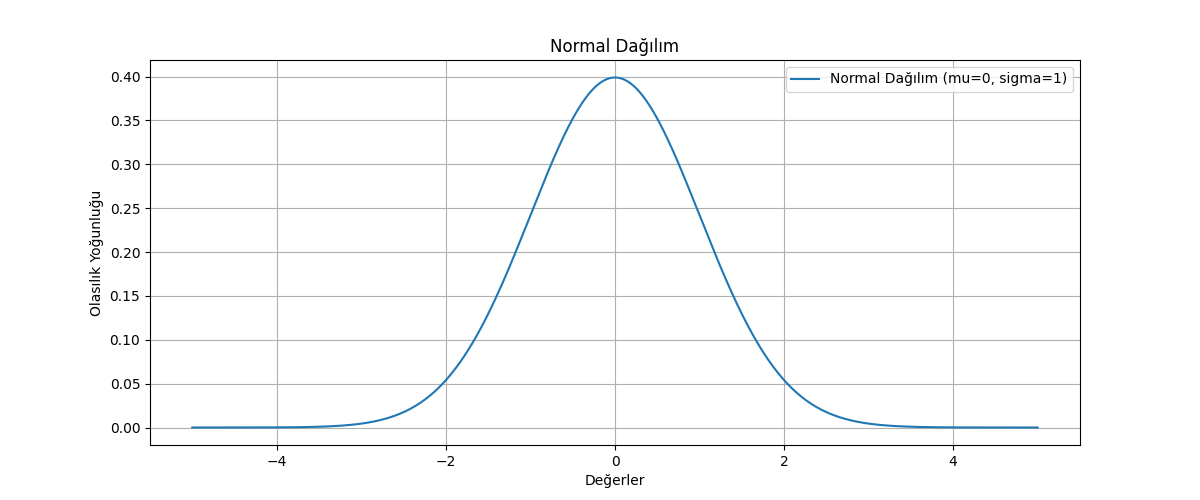
\includegraphics[width=1\textwidth]{images/normal_distribution.png}
    \caption{Normal dağılım örneği.}
    \label{fig:enter-label}
\end{figure}

\subsubsection{Python Kodu}

\begin{lstlisting}[language=Python]
import numpy as np
import matplotlib.pyplot as plt
from scipy.stats import norm

# Normal dagilim parametreleri
mu = 0  # Ortalama
sigma = 1  # Standart sapma

# Normal dagilimi olustur
normal_dist = norm(loc=mu, scale=sigma)

# X araligini belirle
x = np.linspace(-5, 5, 1000)

# Olasilik yogunluk fonksiyonunu hesapla
pdf = normal_dist.pdf(x)

# Grafik cizimi
plt.figure(figsize=(12, 5))
plt.plot(x, pdf, label='Normal Dagilim (mu=0, sigma=1)')
plt.title('Normal Dagilim')
plt.xlabel('Degerler')
plt.ylabel('Olasilik Yogunlugu')
plt.legend()
plt.grid(True)
plt.savefig('normal_distribution')
plt.show()
\end{lstlisting}

\subsubsection{R Kodu}

\begin{lstlisting}[language=R]
dnorm(x = 15 , mean = 34 , sd = 3)

# Bir sinitaki erkeklerin boylarinin ortalamasi 173 cm dir.
# Standart sapma degeri 15 cm ise, secilen bir erkek ogrencinin
# lower.tail FALSE, boyunun 170 cm'den fazla olma olasiligi;
# lower.tail TRUE, boyunun 170 cm'den fazla olmama olasiligi;
pnorm(q = 170, mean = 173, sd = 15, lower.tail = FALSE) # 0.5792
pnorm(q = 170, mean = 173, sd = 15, lower.tail = TRUE) # 0.4207

qnorm(p = 0.90 , mean = 173 , sd = 15 , lower.tail = TRUE) # 192.22

rnorm(n = 50 , mean =  25 , sd = 10)
\end{lstlisting}

\newpage

\subsection{t-Dağılım}
Student t-dağılımı (t-distribution), örneklem büyüklüğü küçük olduğunda ve populasyon standart sapması bilinmediğinde, örneklem ortalamasının dağılımını modellemek için kullanılan bir olasılık dağılımıdır. Özellikle küçük örneklem büyüklüklerinde ve normal dağılım varsayımı sağlanmadığında sıklıkla kullanılır. Student t-dağılımı, William Sealy Gosset tarafından geliştirilmiştir.

\[f(t|n) = \frac{\Gamma\left(\frac{n+1}{2}\right)}{\sqrt{n\pi}\Gamma\left(\frac{n}{2}\right)\left(1+\frac{t^2}{n}\right)^{\frac{n+1}{2}}}\]
\begin{itemize}
	\item $t$: Değer.
	\item $n$: Serbestlik derecesi (örneklem büyüklüğü - 1).
	\item $\Gamma$ Gama fonksiyonu.
\end{itemize}

\begin{figure}[h]
    \centering
    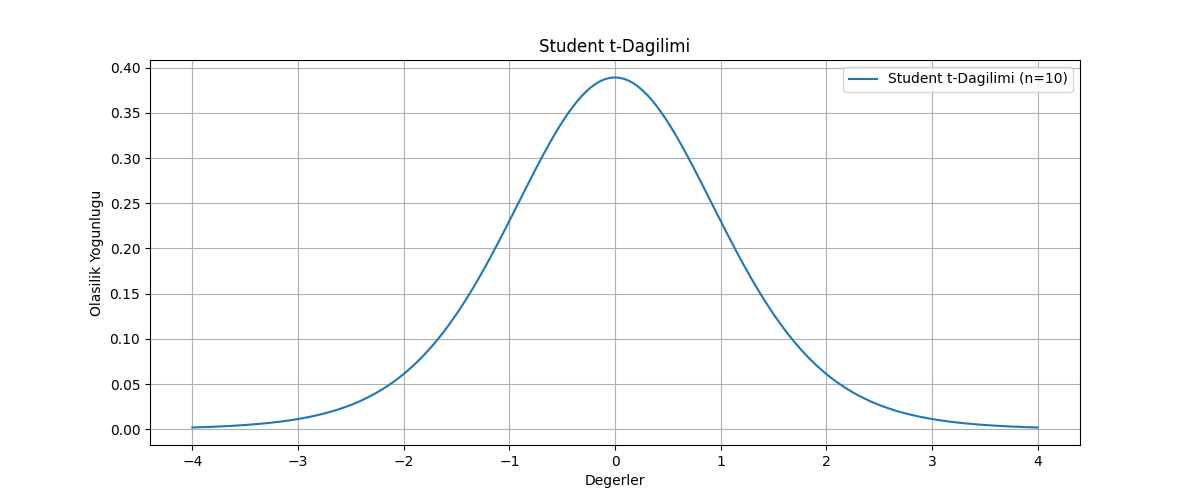
\includegraphics[width=1\textwidth]{images/t_distribution.png}
    \caption{t-dağılım örneği.}
    \label{fig:enter-label}
\end{figure}

\subsubsection{Python Kodu}

\begin{lstlisting}[language=Python]
import numpy as np
import matplotlib.pyplot as plt
from scipy.stats import t

# Serbestlik derecesi (orneklem buyuklugu - 1)
n = 10

# Student t-dagilimini olustur
t_dist = t(df=n)

# X araligini belirle
x = np.linspace(-4, 4, 1000)

# Olasilik yogunluk fonksiyonunu hesapla
pdf = t_dist.pdf(x)

# Grafik cizimi
plt.figure(figsize=(12, 5))
plt.plot(x, pdf, label='Student t-Dagilimi (n=10)')
plt.title('Student t-Dagilimi')
plt.xlabel('Degerler')
plt.ylabel('Olasilik Yogunlugu')
plt.legend()
plt.grid(True)
plt.savefig('t_distribution')
plt.show()
\end{lstlisting}

\newpage

\subsection{Ki-kare (Chi-square) Dağılımı}
Ki-kare dağılımı, bağımsız olarak ve aynı standart normal dağılıma sahip olan rastgele değişkenlerin karelerinin toplamı olarak tanımlanan bir olasılık dağılımıdır. Genellikle hipotez testlerinde ve dağılım karşılaştırmalarında kullanılır.

\[f(x|k) = \frac{1}{2^{\frac{k}{2}} \Gamma\left(\frac{k}{2}\right)} x^{\frac{k}{2} - 1} e^{-\frac{x}{2}}\]
\begin{itemize}
	\item $x$: Değer.
	\item $k$: Serbestlik derecesi.
	\item $\Gamma$: Gama fonksiyonu.
\end{itemize}

\begin{figure}[h]
    \centering
    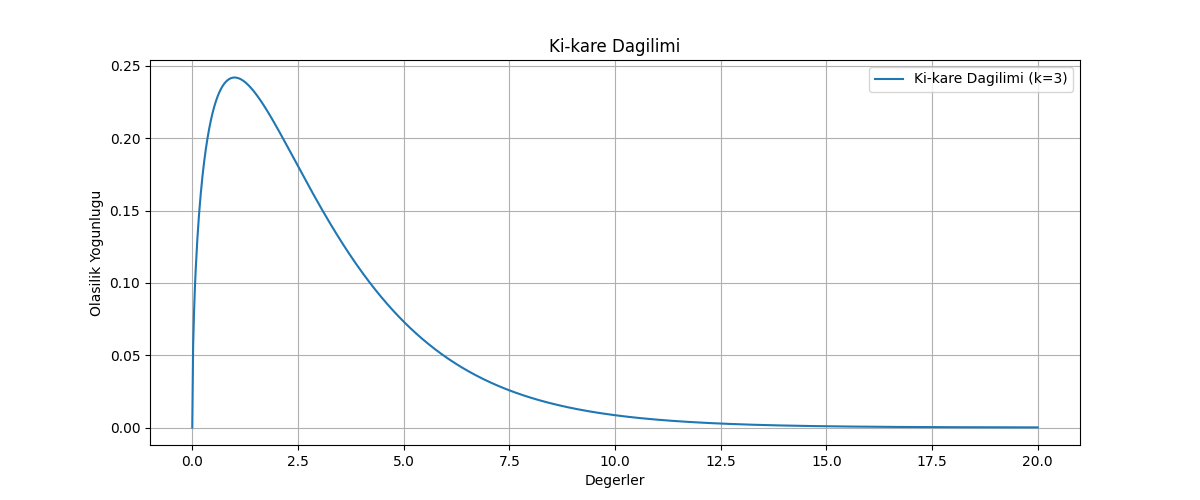
\includegraphics[width=1\textwidth]{images/chi_square_distribution.png}
    \caption{Ki-kare (Chi-square) dağılım örneği.}
    \label{fig:enter-label}
\end{figure}

\subsubsection{Python Kodu}

\begin{lstlisting}[language=Python]
import numpy as np
import matplotlib.pyplot as plt
from scipy.stats import chi2

# Serbestlik derecesi
k = 3

# Ki-kare dagilimini olustur
chi2_dist = chi2(df=k)

# X araligini belirle
x = np.linspace(0, 20, 1000)

# Olasilik yogunluk fonksiyonunu hesapla
pdf = chi2_dist.pdf(x)

# Grafik cizimi
plt.figure(figsize=(12, 5))
plt.plot(x, pdf, label='Ki-kare Dagilimi (k=3)')
plt.title('Ki-kare Dagilimi')
plt.xlabel('Degerler')
plt.ylabel('Olasilik Yogunlugu')
plt.legend()
plt.grid(True)
plt.savefig('chi_square_distribution')
plt.show()
\end{lstlisting}

\newpage

\subsection{Üstel (Exponential) Dağılım}
Üstel dağılım (exponential distribution), belirli bir olayın gerçekleşmesi arasındaki zaman aralığını modellemek için kullanılan bir olasılık dağılımıdır. Özellikle rastgele değişkenin pozitif değerler alması gerektiğinde kullanılır ve genellikle sürekli zaman aralıklarını modellemek için tercih edilir. Üstel dağılım, özellikle rastgele olayların aralıklarının dağılımını modellemek için sıkça kullanılır. Belirli bir olay meydana gelene kadar geçen süre ile ilgilenir. Poisson dağılımı ile aynı parametre olan lambda'yı kullanırlar. Fakat poisson sabit bir zaman aralığına göre bir olayın belirli sayıda meydana gelme olasılığını hesaplarken, üstel dağılım sabit zaman aralığında gerçekleşen olaylarda bir sonraki olayın ne zaman ve ne kadar olasılıkla meydana gelmesiyle ilgilenir.

\[f(x | \lambda) = \lambda * \epsilon ^{-\lambda * \epsilon}\]
\begin{itemize}
	\item $x$: Değer
	\item $\lambda$: Pozitif olan oran parametresi.
\end{itemize}

\begin{figure}[h]
    \centering
    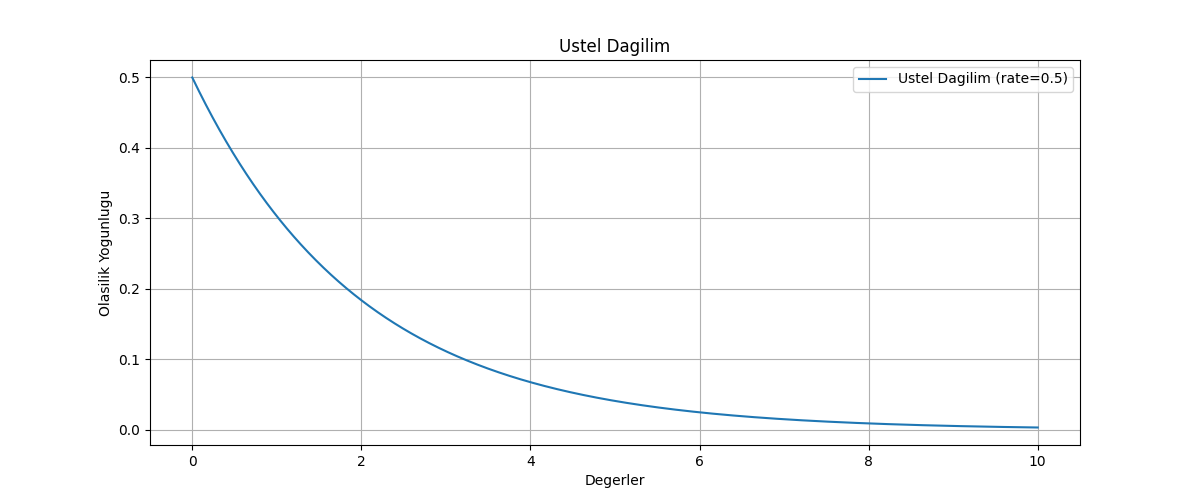
\includegraphics[width=1\textwidth]{images/exponential_distribution.png}
    \caption{Üstel (Exponential) dağılım örneği.}
    \label{fig:enter-label}
\end{figure}

\subsubsection{Python Kodu}

\begin{lstlisting}[language=Python]
import numpy as np
import matplotlib.pyplot as plt
from scipy.stats import expon

# Ustel dagilim parametresi
rate = 0.5  # Oran parametresi (lambda)

# Ustel dagilimi olustur
exponential_dist = expon(scale=1/rate)

# X araligini belirle
x = np.linspace(0, 10, 1000)

# Olasilik yogunluk fonksiyonunu hesapla
pdf = exponential_dist.pdf(x)

# Grafik cizimi
plt.figure(figsize=(12, 5))
plt.plot(x, pdf, label='Ustel Dagilim (rate=0.5)')
plt.title('Ustel Dagilim')
plt.xlabel('Degerler')
plt.ylabel('Olasilik Yogunlugu')
plt.legend()
plt.grid(True)
plt.savefig('exponential_distribution')
plt.show()
\end{lstlisting}

\subsubsection{R Kodu}

\begin{lstlisting}[language=R]
dexp(x = 2 , rate = 1/10)

pexp(5  , rate = 1/10 , lower.tail = TRUE)
pexp(5  , rate = 1/10 , lower.tail = FALSE)

qexp( p = 0.2 , rate = 1/20 , lower.tail = TRUE)

rexp(n = 50 , rate = 1/10)
\end{lstlisting}

\newpage

\subsection{Bernoulli Dağılımı}
İsveçli Bilim adamı Jacop Bernoulli tarafından bulunmuştur. Bernoulli dağılımı, sadece iki olası sonuçtan birini (başarı veya başarısızlık) modellemek için kullanılan bir olasılık dağılımıdır. Özellikle bir denemenin başarılı olma olasılığını (genellikle p ile gösterilir) modellemek için kullanılır. Tek denemede gerçekleşen olayların olasılığının hesaplanmasında kullanılır.

\[f(k|p) = \begin{cases} p & \text{if } k = 1 \\ 1 - p & \text{if } k = 0 \end{cases}\]
\begin{itemize}
	\item $k$: Sonuç (1 başarı, 0 başarısızlık).
	\item $p$: Başarı olasılığı.
\end{itemize}

\[
p(x) = p^x (1 - p)^(1- x)
\]

\begin{itemize}
	\item $p$: Başarılı olma olasılığı.
	\item $q$: Başarısız olma olasılığı.
	\item $x$: Denemeler.
\end{itemize}

\begin{figure}[h]
    \centering
    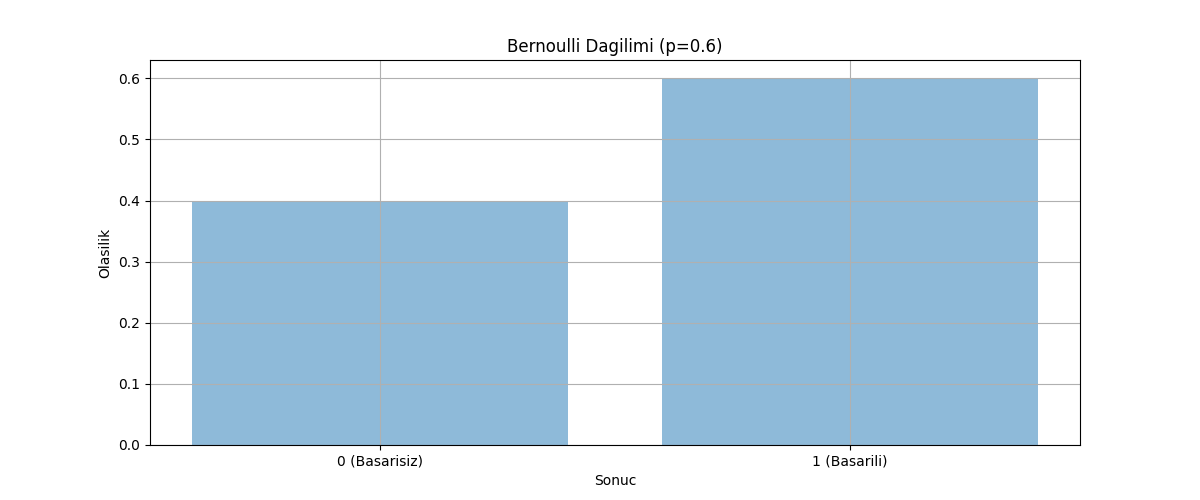
\includegraphics[width=1\textwidth]{images/bernoulli_distribution.png}
    \caption{Bernoulli dağılım örneği.}
    \label{fig:enter-label}
\end{figure}

\subsubsection{Python Kodu}

\begin{lstlisting}[language=Python]
import numpy as np
import matplotlib.pyplot as plt
from scipy.stats import bernoulli

# Basari olasiligi
p = 0.6

# Bernoulli dagilimini olustur
bernoulli_dist = bernoulli(p)

# Degerler
x = [0, 1]

# Olasilik kutle fonksiyonunu hesapla
pmf = bernoulli_dist.pmf(x)

# Grafik cizimi
plt.figure(figsize=(12, 5))
plt.bar(x, pmf, align='center', alpha=0.5)
plt.xticks(x, ['0 (Basarisiz)', '1 (Basarili)'])
plt.title('Bernoulli Dagilimi (p=0.6)')
plt.xlabel('Sonuc')
plt.ylabel('Olasilik')
plt.grid(True)
plt.savefig('bernoulli_distribution')
plt.show()
\end{lstlisting}

\subsubsection{R Kodu}

\begin{lstlisting}[language=R]
library('Rlab')

# dbern, verilen x degerine bu x olasiginin gerceklesme ihtimali bulur.
# x sadece 0 ve 1 olabilir.
dbern(x = 0, prob = 0.7) # 1 - 0.7 = 0.3
dbern(x = 1, prob = 0.7) # 0.7

# lower.tail TRUE, q ve q'dan daha az olma olasiligi.
# lower.tail FALSE, q'dan daha fazla olma olasigi.
# Bernoulli sadece 0 ve 1 girdi aldigi 0-1 arasi.
# pbern, dbern'den cikan sonuclarin toplami.
pbern(q  = 1, prob = 0.7, lower.tail = TRUE) # 1
pbern(q  = 1, prob = 0.7, lower.tail = FALSE) # 0
pbern(q  = 0, prob = 0.7, lower.tail = TRUE) # 0.3
pbern(q  = 0, prob = 0.7, lower.tail = FALSE) # 0.7

# qbern, p degerine gore elde edilecek sonucu bulur.
qbern(p = 0.5, prob = 0.7, lower.tail = TRUE) # 1
qbern(p = 0.2, prob = 0.7, lower.tail = TRUE) # 0
qbern(p = 0.2, prob = 0.7, lower.tail = FALSE) # 1

# rbern, r rastgele bernoulli dagilimi olusturur.
rbern(n = 10, prob = 0.7)
\end{lstlisting}

\newpage

\subsection{Binom (Binomial) Dağılım}
Binom dağılımı, bir denemede başarı veya başarısızlık gibi iki olası sonuç bulunan bağımsız ve aynı dairelerin ardışık olarak tekrarlanması sonucu oluşan bir olasılık dağılımıdır. Her bir denemenin sonucu bağımsızdır ve aynı başarı olasılığına sahiptir. Binom dağılımı, belirli bir sayıda başarı sayısını (başarıların sayısı) modellemek için kullanılır. Bir Bernoulli denemesinin aynı şartlar alında n kez tekrarlanması ile oluşan deneye binom deneyi denir. Binom deneyinin özellikleri;
\begin{itemize}
	\item Deney süresince örneklemdeki deneme sayısı veya denek sayısı değişmez olmalıdır.
	\item Denemeler birbirinden bağımsızdır ve her denemedeki iki olası sonuç vardır.
	\item Her denemede istenilen olay olasığı değişmezdir. Dolayısıyla istenmeyen olay olasılığı $q = 1 - p$ de değişmezdir.
\end{itemize}

\[f(k|n,p) = \binom{n}{k} p^k (1-p)^{n-k}\]
\begin{itemize}
	\item $k$: Başarı sayısı.
	\item $n$: Deneme sayısı.
	\item $p$: Her bir denemenin başarı olasılığı.
	\item $\binom{n}{k}$: n deneme içinden k başarılı deneme seçmek için kombinasyon sayısı.
\end{itemize}

\[
f(x) = p(X = x) = \binom{n}{k} p^x q^(n - x), x = 1,2,3...n
\]

\begin{figure}[h]
    \centering
    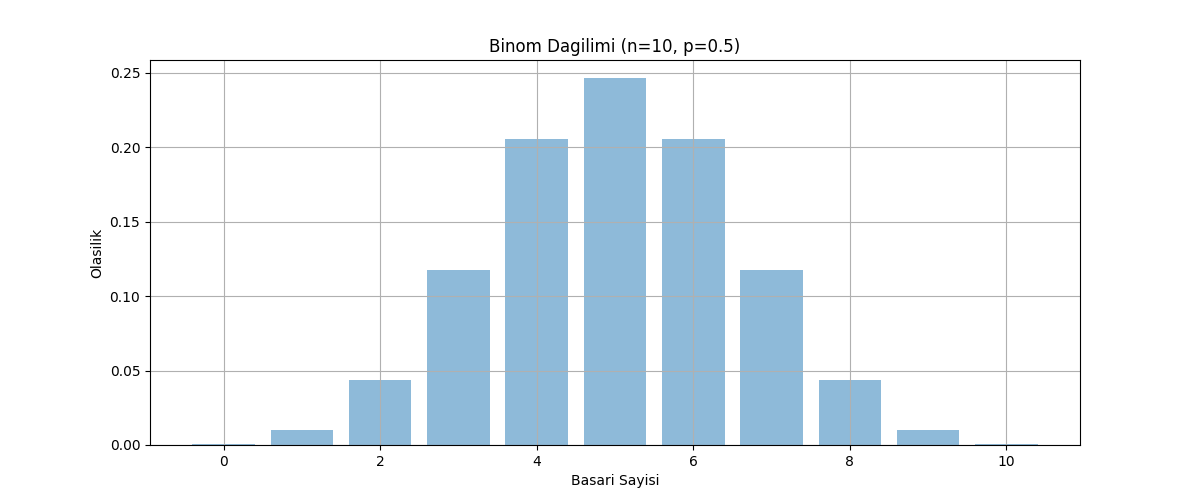
\includegraphics[width=1\textwidth]{images/binomial_distribution.png}
    \caption{Binomial dağılım örneği.}
    \label{fig:enter-label}
\end{figure}

\subsubsection{Python Kodu}

\begin{lstlisting}[language=Python]
import numpy as np
import matplotlib.pyplot as plt
from scipy.stats import binom

# Deneme sayisi
n = 10

# Basari olasiligi
p = 0.5

# Binom dagilimini olustur
binom_dist = binom(n, p)

# Degerler
k = np.arange(0, n+1)

# Olasilik kutle fonksiyonunu hesapla
pmf = binom_dist.pmf(k)

# Grafik cizimi
plt.figure(figsize=(12, 5))
plt.bar(k, pmf, align='center', alpha=0.5)
plt.title('Binom Dagilimi (n=10, p=0.5)')
plt.xlabel('Basari Sayisi')
plt.ylabel('Olasilik')
plt.grid(True)
plt.savefig('binomial_distribution')
plt.show()
\end{lstlisting}

\subsubsection{R Kodu}

\begin{lstlisting}[language=R]
# Basarili olma olasiligi 0.7,
# Basarisiz olma olasiligi 0.3
# 5 kere basarili olma olasiligi;
# dbinom, tekil olasiliklari bulur.
dbinom(x = 5, size = 10, prob = 0.7) # 0.1029

# lower.tail TRUE ise, 5 ve 5'ten daha az basarili olma olasiligi.
# lower.tail FALSE ise, 5'ten daha fazla olma olasiligi.
pbinom(q = 5, size = 30, prob = 0.7, lower.tail = TRUE) # 2.20e-09
pbinom(q = 5, size = 30, prob = 0.7, lower.tail = FALSE) # 0.99

# Bir e-ticaret sitesine gelen 5 musteriden 1'i
# siparis veriyor. Birgunde 50 musterinin
# siteye girmesi bekleniyorsa en az 10 siparis
# alma olasiligi kactir ?
pbinom(q = 10 - 1, size = 50, prob = 1/5, lower.tail = FALSE) # 0.55

# rastgele binom dagilimi
rbinom(n = 50 , size = 30 , prob = 1/4)
\end{lstlisting}

\newpage

\subsection{Tekdüze (Uniform) Dağılım}
Uniform (düzgün) dağılım, belirli bir aralıktaki tüm değerlerin eşit olasılıkla ortaya çıkma durumunu modelleyen bir olasılık dağılımıdır. Bu dağılım, belirli bir aralıktaki rastgele değişkenlerin dağılımını ifade etmek için kullanılır. Uniform dağılım hem kesikli hem de sürekli olabilir.

\[f(x|a,b) = \frac{1}{b-a}\]
\begin{itemize}
	\item $x$: Değer.
	\item $a$: Dağılımın başlangıç noktası (alt sınır).
	\item $b$: Dağılımın bitiş noktası (üst sınır).
\end{itemize}

\begin{figure}[h]
    \centering
    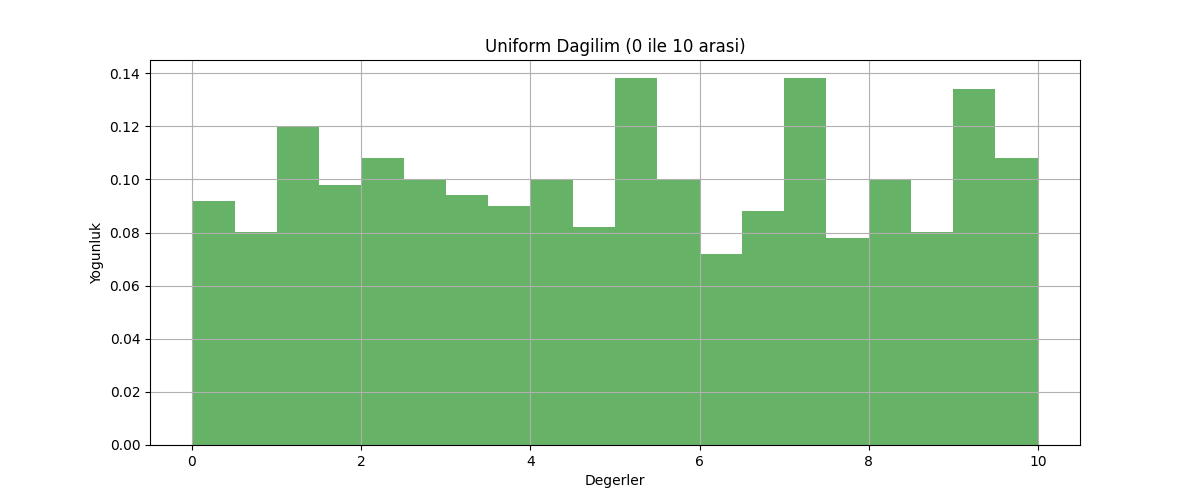
\includegraphics[width=0.8\textwidth]{images/uniform_distribution.png}
    \caption{Tekdüze (uniform) dağılım örneği.}
    \label{fig:enter-label}
\end{figure}

\subsubsection{Python Kodu}

\begin{lstlisting}[language=Python]
import numpy as np
import matplotlib.pyplot as plt

# Uniform dagilimin parametreleri (0 ile 10 arasi)
a = 0  # Alt sinir
b = 10  # Ust sinir

# Ornek veri seti olustur
uniform_data = np.random.uniform(a, b, 1000)

# Grafik cizimi
plt.figure(figsize=(12, 5))
plt.hist(uniform_data, bins=20, density=True, alpha=0.6, color='g')
plt.title('Uniform Dagilim (0 ile 10 arasi)')
plt.xlabel('Degerler')
plt.ylabel('Yogunluk')
plt.grid(True)
plt.savefig('uniform_distribution')
plt.show()
\end{lstlisting}

\subsubsection{R Kodu}

\begin{lstlisting}[language=R]
dunif(x = 5, min = 0, max = 10)

punif(q = 4, min = 0, max = 10, lower.tail = TRUE)
punif(q = 4, min = 0, max = 10, lower.tail = TRUE)

qunif(p = 0.80, min = 0, max = 20, lower.tail = TRUE)
qunif(p = 0.80, min = 0, max = 20, lower.tail = FALSE)

runif(n = 5, min = 1, max = 10)
\end{lstlisting}

\newpage

\subsection{Poisson Dağılımı}
Poisson dağılımı, sabit bir zaman biriminde belirli bir alanda veya hacimde nadir rastgele olayların (örneğin, trafik kazaları, doğal afetler, müşteri hizmet çağrıları vb.) sayısını modellemek için kullanılan bir olasılık dağılımıdır. Poisson dağılımı, belirli bir zaman veya alanda olayların ortalamasını (örneğin, ortalama bir saatteki trafik kazaları sayısı) ve olayların beklenen nadirliğini temel alır. Poisson deneyinde;

\begin{enumerate}
	\item Bütün eylemler birbirinden bağımsız olmalıdır.
	\item Her olay için bir zaman aralığı sabit olmalıdır.
	\item İki olay aynı anda gerçekleşemez.
\end{enumerate}

\[f(k|\lambda) = \frac{e^{-\lambda} \lambda^k}{k!}\]
\begin{itemize}
	\item $k$: Olay sırası.
	\item $\lambda$: Olayların ortalama sayısı.
	\item $\epsilon$: Euler sayısı.
\end{itemize}

\begin{figure}[h]
    \centering
    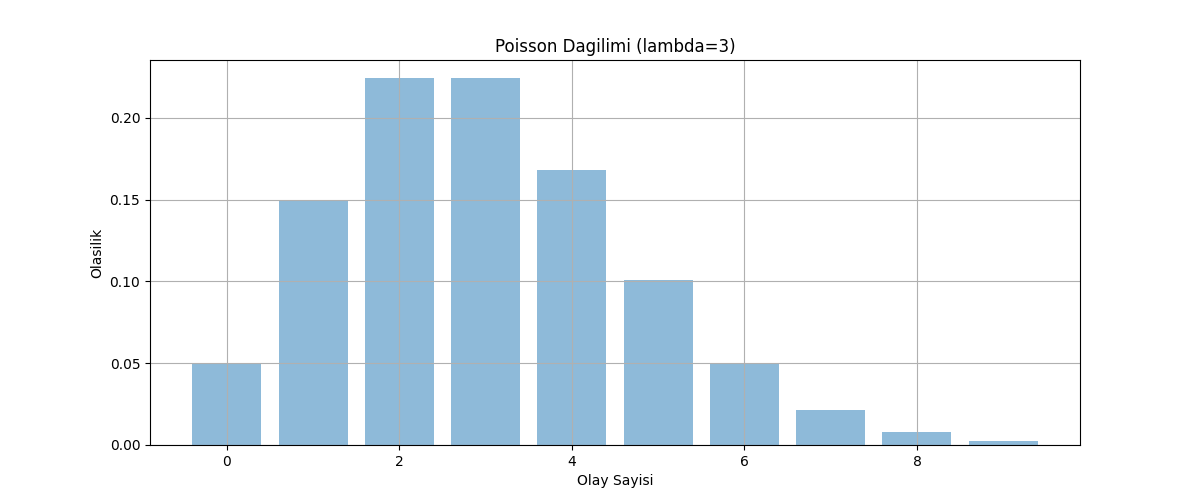
\includegraphics[width=0.8\textwidth]{images/poisson_distribution.png}
    \caption{Poisson dağılım örneği.}
    \label{fig:enter-label}
\end{figure}

\subsubsection{Python Kodu}

\begin{lstlisting}[language=Python]
import numpy as np
import matplotlib.pyplot as plt
from scipy.stats import poisson

# Olaylarin ortalama sayisi (lambda)
lam = 3

# Poisson dagilimini olustur
poisson_dist = poisson(mu=lam)

# Degerler
k = np.arange(0, 10)

# Olasilik kutle fonksiyonunu hesapla
pmf = poisson_dist.pmf(k)

# Grafik cizimi
plt.figure(figsize=(12, 5))
plt.bar(k, pmf, align='center', alpha=0.5)
plt.title('Poisson Dagilimi (lambda=3)')
plt.xlabel('Olay Sayisi')
plt.ylabel('Olasilik')
plt.grid(True)
plt.savefig('poisson_distribution')
plt.show()
\end{lstlisting}

\subsubsection{R Kodu}

\begin{lstlisting}[language=R]
# 1 saatte 5 araba gecme olasiligi:
dpois(x = 5, lambda = 15) # 0.0019

# 1 dakikada 2 araba gecme olasiligi;
# 60 dakikada 20 ise
# 1 dakikada 20/60 = lambda = 1/3.
ppois(q = 2, lambda = 1/3, lower.tail = TRUE) # 0.995
ppois(q = 2, lambda = 1/3, lower.tail = FALSE) # 0.004
\end{lstlisting}

\newpage

\subsection{Hipergeometrik  Dağılım}
Hipergeometrik dağılım bir sonlu popülasyon içerisinden rastgele ve geri koymadan seçilen örneklemler arasındaki başarı sayısını hesaplamak için kulllanılır. 

\[
P(X = k) = \frac{\binom{K}{k} \binom{N-K}{n-k}}{\binom{N}{n}}
\]

\begin{itemize}
	\item $N$: Öğe sayısı.
	\item $K$: Başarı.
	\item $n$: Örneklem büyüklüğü.
	\item $k$: Başarı olasılığı.
	\item $\binom{K}{k}$: K başarıdan k tanesini seçmenin kombinasyon sayısı.
	\item $\binom{N-K}{n-k}$: N - K başarısızlıktan n - k tanesini seçmenin kombinasyon sayısı.
	\item $\binom{N}{n}$: N öğeden n tanesini seçmenin toplam kombinasyon sayısı.
\end{itemize}

\subsubsection{R Kodu}

\begin{lstlisting}[language=R]
# 26 kirmizi ve 24 sari kart olmak uzere
# Secilen 10 tanesinden 4'u kirmizi kart olma olasiligi;
dhyper(x = 4, m = 26, n = 24, k = 10) # 0.1958

# lower.tail TRUE, en fazla 4 kirmizi kart,
# lower.tail FALSE, en az 4 kirmizi kart.
phyper(q = 4, m = 26, n = 24, k = 10, lower.tail = TRUE) # 0.31
phyper(q = 4, m = 26, n = 24, k = 10, lower.tail = FALSE) # 0.68

# rastgele hipergeometrik dagilim
rhyper(nn = 50 , m = 20 , n = 12, k = 10)
\end{lstlisting}

\newpage 